% Options for packages loaded elsewhere
\PassOptionsToPackage{unicode}{hyperref}
\PassOptionsToPackage{hyphens}{url}
\PassOptionsToPackage{dvipsnames,svgnames,x11names}{xcolor}
%
\documentclass[
]{template/style/uneceart}

\usepackage{amsmath,amssymb}
\usepackage{iftex}
\ifPDFTeX
  \usepackage[T1]{fontenc}
  \usepackage[utf8]{inputenc}
  \usepackage{textcomp} % provide euro and other symbols
\else % if luatex or xetex
  \usepackage{unicode-math}
  \defaultfontfeatures{Scale=MatchLowercase}
  \defaultfontfeatures[\rmfamily]{Ligatures=TeX,Scale=1}
\fi
\usepackage{lmodern}
\ifPDFTeX\else  
    % xetex/luatex font selection
\fi
% Use upquote if available, for straight quotes in verbatim environments
\IfFileExists{upquote.sty}{\usepackage{upquote}}{}
\IfFileExists{microtype.sty}{% use microtype if available
  \usepackage[]{microtype}
  \UseMicrotypeSet[protrusion]{basicmath} % disable protrusion for tt fonts
}{}
\makeatletter
\@ifundefined{KOMAClassName}{% if non-KOMA class
  \IfFileExists{parskip.sty}{%
    \usepackage{parskip}
  }{% else
    \setlength{\parindent}{0pt}
    \setlength{\parskip}{6pt plus 2pt minus 1pt}}
}{% if KOMA class
  \KOMAoptions{parskip=half}}
\makeatother
\usepackage{xcolor}
\setlength{\emergencystretch}{3em} % prevent overfull lines
\setcounter{secnumdepth}{-\maxdimen} % remove section numbering
% Make \paragraph and \subparagraph free-standing
\ifx\paragraph\undefined\else
  \let\oldparagraph\paragraph
  \renewcommand{\paragraph}[1]{\oldparagraph{#1}\mbox{}}
\fi
\ifx\subparagraph\undefined\else
  \let\oldsubparagraph\subparagraph
  \renewcommand{\subparagraph}[1]{\oldsubparagraph{#1}\mbox{}}
\fi


\providecommand{\tightlist}{%
  \setlength{\itemsep}{0pt}\setlength{\parskip}{0pt}}\usepackage{longtable,booktabs,array}
\usepackage{calc} % for calculating minipage widths
% Correct order of tables after \paragraph or \subparagraph
\usepackage{etoolbox}
\makeatletter
\patchcmd\longtable{\par}{\if@noskipsec\mbox{}\fi\par}{}{}
\makeatother
% Allow footnotes in longtable head/foot
\IfFileExists{footnotehyper.sty}{\usepackage{footnotehyper}}{\usepackage{footnote}}
\makesavenoteenv{longtable}
\usepackage{graphicx}
\makeatletter
\def\maxwidth{\ifdim\Gin@nat@width>\linewidth\linewidth\else\Gin@nat@width\fi}
\def\maxheight{\ifdim\Gin@nat@height>\textheight\textheight\else\Gin@nat@height\fi}
\makeatother
% Scale images if necessary, so that they will not overflow the page
% margins by default, and it is still possible to overwrite the defaults
% using explicit options in \includegraphics[width, height, ...]{}
\setkeys{Gin}{width=\maxwidth,height=\maxheight,keepaspectratio}
% Set default figure placement to htbp
\makeatletter
\def\fps@figure{htbp}
\makeatother
\newlength{\cslhangindent}
\setlength{\cslhangindent}{1.5em}
\newlength{\csllabelwidth}
\setlength{\csllabelwidth}{3em}
\newlength{\cslentryspacingunit} % times entry-spacing
\setlength{\cslentryspacingunit}{\parskip}
\newenvironment{CSLReferences}[2] % #1 hanging-ident, #2 entry spacing
 {% don't indent paragraphs
  \setlength{\parindent}{0pt}
  % turn on hanging indent if param 1 is 1
  \ifodd #1
  \let\oldpar\par
  \def\par{\hangindent=\cslhangindent\oldpar}
  \fi
  % set entry spacing
  \setlength{\parskip}{#2\cslentryspacingunit}
 }%
 {}
\usepackage{calc}
\newcommand{\CSLBlock}[1]{#1\hfill\break}
\newcommand{\CSLLeftMargin}[1]{\parbox[t]{\csllabelwidth}{#1}}
\newcommand{\CSLRightInline}[1]{\parbox[t]{\linewidth - \csllabelwidth}{#1}\break}
\newcommand{\CSLIndent}[1]{\hspace{\cslhangindent}#1}

\usepackage{booktabs}
\usepackage{longtable}
\usepackage{array}
\usepackage{multirow}
\usepackage{wrapfig}
\usepackage{float}
\usepackage{colortbl}
\usepackage{pdflscape}
\usepackage{tabu}
\usepackage{threeparttable}
\usepackage{threeparttablex}
\usepackage[normalem]{ulem}
\usepackage{makecell}
\usepackage{xcolor}
\usepackage{template/style/UNECE2023}
\usepackage{enumerate}
\usepackage{xcolor}
\usepackage{float}
\floatplacement{table}{b}
\definecolor{unece_color}{RGB}{84, 141, 212}

%% the title of your contribution in capital letters:
\newcommand{\TITLE}{\textbf{ASSESSING THE UTILITY OF SYNTHETIC DATA: A DENSITY RATIO PERSPECTIVE} \\}

%% author:
\newcommand{\AUTHOR}{Thom Benjamin Volker (Utrecht University, the Netherlands; Statistics Netherlands, the Netherlands)\\Peter-Paul de Wolf (Statistics Netherlands, the Netherlands)\\Erik-Jan van Kesteren (Utrecht University, the Netherlands)}

%% your organisation
% \newcommand{\ORGANISATION}{\textsuperscript{1} (Utrecht University, the Netherlands), \textsuperscript{2} (Statistics Netherlands, the Netherlands)}
\newcommand{\EMAIL}{\href{mailto:t.b.volker@uu.nl}{t.b.volker@uu.nl}, \href{mailto:pp.dewolf@cbs.nl}{pp.dewolf@cbs.nl}, \href{mailto:e.vankesteren1@uu.nl}{e.vankesteren1@uu.nl}}

%% abstract
\newcommand{\ABSTRACT}{Synthetic data can be a solution to reduce disclosure risks that arise when disseminating research data to the public. However, for the synthetic data to be useful for general inferential purposes, it is paramount that its distribution is similar to the distribution of the observed data. Often, data disseminators consider multiple synthetic data models and make refinements in an iterative fashion. After each adjustment, it is crucial to evaluate whether the quality of the synthetic data has actually improved. Although many methods exist to provide such an evaluation, their results are often incomplete or even misleading. To improve the evaluation strategy for synthetic data, and thereby the quality of synthetic data itself, we propose to use the density ratio estimation framework. Using techniques from this field, we show how an interpretable utility measure can be obtained from the ratio of the observed and synthetic data densities. We show how the density ratio estimation framework bridges the gap between fit-for-purpose and global utility measures, and discuss how it can also be used to evaluate analysis-specific utility. Using empirical examples, we show that density ratio estimation improves on existing (global) utility measures by providing higher statistical power and offering a fine-grained view of discrepancies between the observed and synthetic data. Moreover, we describe several additional advantages of the approach, such as providing a measure of utility on the level of individual synthetic data points, automatic model selection without requiring user specification, and readily available high-dimensional extensions. We conclude that density ratio estimation provides a promising framework in synthetic data generation workflows and present an R-package with functionality to implement the approach.}


\makeatletter
\makeatother
\makeatletter
\makeatother
\makeatletter
\@ifpackageloaded{caption}{}{\usepackage{caption}}
\AtBeginDocument{%
\ifdefined\contentsname
  \renewcommand*\contentsname{Table of contents}
\else
  \newcommand\contentsname{Table of contents}
\fi
\ifdefined\listfigurename
  \renewcommand*\listfigurename{List of Figures}
\else
  \newcommand\listfigurename{List of Figures}
\fi
\ifdefined\listtablename
  \renewcommand*\listtablename{List of Tables}
\else
  \newcommand\listtablename{List of Tables}
\fi
\ifdefined\figurename
  \renewcommand*\figurename{Figure}
\else
  \newcommand\figurename{Figure}
\fi
\ifdefined\tablename
  \renewcommand*\tablename{Table}
\else
  \newcommand\tablename{Table}
\fi
}
\@ifpackageloaded{float}{}{\usepackage{float}}
\floatstyle{ruled}
\@ifundefined{c@chapter}{\newfloat{codelisting}{h}{lop}}{\newfloat{codelisting}{h}{lop}[chapter]}
\floatname{codelisting}{Listing}
\newcommand*\listoflistings{\listof{codelisting}{List of Listings}}
\makeatother
\makeatletter
\@ifpackageloaded{caption}{}{\usepackage{caption}}
\@ifpackageloaded{subcaption}{}{\usepackage{subcaption}}
\makeatother
\makeatletter
\@ifpackageloaded{tcolorbox}{}{\usepackage[skins,breakable]{tcolorbox}}
\makeatother
\makeatletter
\@ifundefined{shadecolor}{\definecolor{shadecolor}{rgb}{.97, .97, .97}}
\makeatother
\makeatletter
\makeatother
\makeatletter
\makeatother
\ifLuaTeX
  \usepackage{selnolig}  % disable illegal ligatures
\fi
\IfFileExists{bookmark.sty}{\usepackage{bookmark}}{\usepackage{hyperref}}
\IfFileExists{xurl.sty}{\usepackage{xurl}}{} % add URL line breaks if available
\urlstyle{same} % disable monospaced font for URLs
\hypersetup{
  colorlinks=true,
  linkcolor={blue},
  filecolor={Maroon},
  citecolor={Blue},
  urlcolor={Blue},
  pdfcreator={LaTeX via pandoc}}

\author{}
\date{}

\begin{document}
\ifdefined\Shaded\renewenvironment{Shaded}{\begin{tcolorbox}[breakable, frame hidden, interior hidden, boxrule=0pt, sharp corners, borderline west={3pt}{0pt}{shadecolor}, enhanced]}{\end{tcolorbox}}\fi

%%% by Matthias Templ, Vienna University of Technology, March 13, 2012. Updated Frederic Picard, Statistics Canada, March 09, 2015. Updated D. Kilchmann, SFSO, 7.12.2016, 5.4.2018., 8.10.2020, 6.4.2022
%%% Updated by Peter-Paul de Wolf for use in UNECE/Eruostat SDC meetings, 15.03.2023

\setcounter{page}{1}
\thispagestyle{empty} \vspace*{-2.0cm} %[width=0.65\textwidth]

\includegraphics[height=1.5cm]{template/UNECE_logo}\hspace*{8cm}
\includegraphics[height=1.5cm]{template/ModernStatsLogo}\\[\baselineskip]
%\hspace*{13cm} Working Paper \\
%\hspace*{13cm}ENGLISH ONLY\\\\
\textsc{UNITED NATIONS ECONOMIC COMMISSION FOR EUROPE} \vspace*{2mm}\\
\textsc{CONFERENCE OF EUROPEAN STATISTICIANS}\vspace*{2mm}\\
\textbf{Expert meeting on Statistical Data Confidentiality}\vspace*{2mm}\\
26--28 September 2023, Wiesbaden              %% check whether it is the right place and date
\vspace*{-1mm}
{\color{unece_color} \par\noindent\rule{\textwidth}{1.25pt}}\\[1cm]
%\TOPIC
%\begin{center}
{\LARGE \TITLE}\vspace*{-2mm}\\ %17pt
%\TYPE
\AUTHOR\ \\%11pt
% \ORGANISATION\vspace{2mm}\\ %11pt
\EMAIL\vspace*{1cm}\\ %11pt
%\end{center}
\noindent
{\large\textbf{\textit{Abstract}}}\\ %12pt
\ABSTRACT
\newpage



\hypertarget{introduction}{%
\section{Introduction}\label{introduction}}

In recent years, the academic interest in synthetic data has exploded.
Synthetic data are increasingly being used as a solution to overcome
privacy and confidentiality issues that are inherently linked to the
dissemination of research data. National statistical institutes and
other government agencies have started to disseminate synthetic data to
the public while restricting access to the original data to protect
sensitive information (e.g.,
\protect\hyperlink{ref-SIPP_Beta_2006}{Abowd, Stinson, and Benedetto
2006}; \protect\hyperlink{ref-hawala_synthetic_2008}{Hawala 2008};
\protect\hyperlink{ref-drechsler2012}{Drechsler 2012}). At the same
time, researchers began to share synthetic versions of their research
data to comply with open science standards (e.g.,
\protect\hyperlink{ref-vandewiel2023}{van de Wiel et al. 2023};
\protect\hyperlink{ref-obermeyer2019}{Obermeyer et al. 2019};
\protect\hyperlink{ref-zettler2021}{Zettler et al. 2021}). Rather than
sharing the original research data, a synthetic surrogate is shared to
facilitate reviewing of the data processing and analysis pipeline.
Additionally, synthetic data is increasingly being used for training
machine learning models (\protect\hyperlink{ref-nikolenko2021}{Nikolenko
2021}). On a lower level, synthetic data can be used in model testing
pipelines (before access to the real data is provided), for data
exploration, and for educational purposes.

At its core, the idea of synthetic data is to replace values from the
observed data with new values that are generated from a model. In this
way, it is possible to generate an entirely new synthetic data set
(commonly referred to as the \emph{fully} synthetic data approach;
\protect\hyperlink{ref-rubin_statistical_1993}{Rubin 1993}), but also to
replace just those values that are sensitive or that would yield a high
risk of disclosure when released (an approach called \emph{partially}
synthetic data; \protect\hyperlink{ref-little_statistical_1993}{Little
1993}). Both approaches attempt to build a model that incorporates as
much of the information in the real data as possible, given a
pre-specified privacy risk level that is still deemed acceptable. The
models used to generate synthetic data were originally closely related
to methods used for multiple imputation of missing data, such as fully
conditional specification (\protect\hyperlink{ref-volker2021}{Volker and
Vink 2021}) or sequential regression
(\protect\hyperlink{ref-nowok2016}{Nowok, Raab, and Dibben 2016}).
Recently, significant improvements in generative modelling sparked the
scientific interest in synthetic data in the computer science community,
leading to novel synthesis methods (e.g.,
\protect\hyperlink{ref-patki2016}{Patki, Wedge, and Veeramachaneni
2016}; \protect\hyperlink{ref-xu_ctgan_2019}{Xu et al. 2019}). Combined
with work on formal privacy guarantees, this resulted in new models that
explicitly control the level of privacy risk in synthesis methods
(\protect\hyperlink{ref-jordon2018pategan}{Jordon, Yoon, and Schaar
2019}; \protect\hyperlink{ref-Torkzadehmahani2019}{Torkzadehmahani,
Kairouz, and Paten 2019}). Through both methodological advances and
practical implementations, data synthesis has evolved into an
increasingly popular approach to enhance data dissemination.

Regardless of these developments, the main challenge when generating
synthetic data remains to adequately balance the privacy risk with the
utility (i.e., quality) of the synthetic data. On the upper limit of
this privacy-utility trade-off, the synthesis model captures the
information in the observed data so precisely that the real data is
exactly reproduced, resulting in the same privacy loss as when
disseminating the real data. In statistical terms, the synthesis model
is overparameterized to such an extent that there are no degrees of
freedom left, and there is thus no randomness involved in the generation
of the synthetic values. On the lower limit of the trade-off, synthetic
values are generated without borrowing any information from the real
data. For example, we could place the value \(0\) or a random draw from
a standard normal distribution for every record and every variable, such
that the synthetic data contains only noise. Synthetic data sets sit
somewhere between these extremes: they contain some information from the
real data, yielding some disclosure risk, but they also resemble the
real data to some extent, yielding more than zero utility. Because not
all information is captured, the utility of the synthetic data will
always be lower than the utility of the real data. The question that
naturally arises is where on the privacy-utility continuum the synthetic
data is located: how much information is sacrificed, and which aspects
of the real data are reproduced in the synthetic data. From the
perspective of the data provider, it is important to know how
informative the released data is, while the user wants to know whether
their analysis can be reliably performed. Additionally, the data
provider can use knowledge about the utility to finetune the synthesis
model and improve the synthetic data quality.

To evaluate the utility of synthetic data, three classes of utility
measures have been distinguished (for a thorough review of these
measures, see \protect\hyperlink{ref-drechsler2023}{Drechsler and
Haensch 2023}): fit-for-purpose measures, global utility measures, and
analysis-specific utility measures. Fit-for-purpose measures are often
the first step in assessing the quality of the synthetic data. They
typically involve comparing the univariate distributions of the observed
and synthetic data (for example using visualization techniques or
goodness-of-fit measures). Although these measures provide an initial
impression of the quality of the synthesis models used, this picture is
by definition limited, because only one or two variables are assessed at
the same time. Hence, complex relationships between variables will
always be out of scope. Global utility measures build on the
fit-for-purpose measures, but attempt to capture the quality of the
entire multivariate distribution of the synthetic data relative to the
observed data in a single, global, indicator. This can be done using
some distance measure (e.g., the Kullback-Leibler divergence; see
\protect\hyperlink{ref-karr_utility_2006}{Karr et al. 2006}), but also
by estimating how well a prediction model can distinguish between the
observed and synthetic data, using the predicted probabilities
(propensity scores;
\protect\hyperlink{ref-rosenbaum_propensity_scores_1983}{Rosenbaum and
Rubin 1983}) as a measure of discrepancy (e.g., the propensity score
mean squared error, \(pMSE\);
\protect\hyperlink{ref-Woo_global_2009}{Woo et al. 2009};
\protect\hyperlink{ref-snoke_utility_2018}{Snoke et al. 2018}). While
global utility measures paint a rather complete picture, and provide
information over the entire range of the data, they tend to be too
general. That is, global utility measures can be so broad that important
discrepancies between the real and synthetic are missed, and a synthetic
data set with high global utility might still yield analyses with
results that are far from the results from real data analyses (see
\protect\hyperlink{ref-drechsler_utility_2022}{Drechsler 2022}). Lastly,
the analysis-specific utility measures quantify to what extent analyses
performed on the synthetic data align with the same analyses on the
observed data. These measures can, for example, evaluate how similar the
coefficients of a regression model are (e.g., using the confidence
interval overlap; \protect\hyperlink{ref-karr_utility_2006}{Karr et al.
2006}), or whether prediction models trained on the synthetic and
observed data perform comparably in terms of evaluation metrics.
However, analysis-specific utility generally does not carry over: high
specific utility for one analysis does not at all imply high utility for
another analysis. Since data providers typically do not know which
analyses will be performed with the synthetic data, it is impossible to
provide analysis-specific utility measures for all potentially relevant
analyses (see also
\protect\hyperlink{ref-drechsler_utility_2022}{Drechsler 2022}).

In this paper, we propose to use the framework of density ratio
estimation
(\protect\hyperlink{ref-sugiyama_suzuki_kanamori_2012}{Sugiyama, Suzuki,
and Kanamori 2012a}) to place all above measures under a common
umbrella. We show empirically that this approach performs at least as
well as various existing utility measures, while providing a more
fine-grained view of the misfit of the synthetic data. Moreover, the
typically non-parametric nature of density ratio estimation in
combination with automatic model selection mitigates the burden around
model specification of existing utility measures as the \(pMSE\). In
short, density ratio estimation compares the (multivariate)
distributions of two data sets (e.g., two different samples or groups)
by directly estimating the ratio of their densities. Crucially, this
method does not estimate the densities of the observed and synthetic
data separately, subsequently taking their ratio, but estimates the
density ratio directly, which has been shown to yield better performance
(e.g., \protect\hyperlink{ref-kanamori_ulsif_2009}{Kanamori, Hido, and
Sugiyama 2009}). The idea is that if two data sets are drawn from the
same data-generating mechanism, the sampled data should be similar, and
the ratio of their densities should be close to one over the entire
multivariate space. This approach readily extends from univariate to
bivariate and multivariate densities, and thus bridges the gap between
fit-for-purpose and global utility measures. Moreover, we briefly
discuss how density ratio estimation can be used to compare the
distributions of parameters of observed and synthetic data, to
incorporate analysis-specific utility measures as well. Hence, we show
that it is a versatile approach that is useful in the entire domain of
data utility.

Also from the privacy-side several promising advances have been made to
quantify the amount of information leakage through the synthetic data.
Important work has been done to build formal privacy guarantees into the
synthesis models through differential privacy
(\protect\hyperlink{ref-dwork_dp_2006}{Dwork 2006}). In addition to
these privacy-by-design mechanisms, some measures exist to quantify
privacy loss of synthetic data after generation (e.g.,
\protect\hyperlink{ref-mcclure2016assessing}{McClure and Reiter 2016};
\protect\hyperlink{ref-Reiter_Mitra_2009}{Reiter and Mitra 2009};
\protect\hyperlink{ref-hu2019}{Hu 2019}). However, the practical
applicability of these measures depends on whether the data is fully or
partially synthetic, and especially in case of the former, the practical
applicability of these measures is often limited (for an extensive
discussion of these issues, see
\protect\hyperlink{ref-drechsler2023}{Drechsler and Haensch 2023}). More
research on measures to evaluate disclosure risks in synthetic data is
thus certainly needed, but in this paper we focus exclusively on
measuring utility.

In what follows, we describe the density ratio estimation framework by
summarizing some of the work in this area, and show how it provides a
useful framework for measuring utility of synthetic data. Subsequently,
we illustrate how the method can be used in practice by providing
multiple examples, and empirically compare its performance to existing
utility measures. Lastly, we discuss how density ratio estimation
relates to existing utility measures, describe current shortcomings of
the approach and relate these shortcomings to avenues for future work.

\hypertarget{density-ratio-estimation}{%
\section{Density ratio estimation}\label{density-ratio-estimation}}

The density ratio estimation framework was originally developed in the
machine learning community for the comparison of two probability
distributions (for an overview, see
\protect\hyperlink{ref-sugiyama_suzuki_kanamori_2012}{Sugiyama, Suzuki,
and Kanamori 2012a}). The framework has been shown to be applicable to
prediction (\protect\hyperlink{ref-sugiyama_conditional_2010}{Sugiyama
et al. 2010};
\protect\hyperlink{ref-sugiyama_classification_2010}{Sugiyama 2010}),
outlier detection (\protect\hyperlink{ref-shohei_dre_outlier_2008}{Hido
et al. 2008}), change-point detection in time-series
(\protect\hyperlink{ref-liu_change_2013}{Liu et al. 2013}), importance
weighting under domain adaptation (i.e., sample selection bias;
\protect\hyperlink{ref-kanamori_ulsif_2009}{Kanamori, Hido, and Sugiyama
2009}), and, importantly, two-sample homogeneity tests
(\protect\hyperlink{ref-sugiyama_lstst_2011}{Sugiyama, Suzuki, et al.
2011}). The general idea of density ratio estimation is depicted in
Figure~\ref{fig-dr-plot}, and boils down to comparing two distributions
by modelling the density ratio \(r(\boldsymbol{x})\) between the
probability distributions of the numerator samples, taken from the
synthetic data distribution, \(p_{syn}(\boldsymbol{x})\), and the
denominator samples, taken from the observed data distribution,
\(p_{obs}(\boldsymbol{x})\), such that
\begin{equation}\protect\hypertarget{eq-dr}{}{
r(\boldsymbol{x}) = \frac{p_{syn}(\boldsymbol{x})}{p_{obs}(\boldsymbol{x})}.
}\label{eq-dr}\end{equation} This specification has the intuitive
interpretation that if the density ratio is large, too many synthetic
values will be generated in that region, whereas if the density ratio is
small, there will be too few synthetic observations, both relative to
the observed data. An intuitive approach to estimating
\(r(\boldsymbol{x})\) from samples of \(p_{obs}(\boldsymbol{x})\) and
\(p_{syn}(\boldsymbol{x})\) would be to estimate the observed and
synthetic data density separately, for example using kernel density
estimation (\protect\hyperlink{ref-Scott1992}{Scott 1992}), and
subsequently compute the ratio of these estimated densities. However,
density estimation is one of the hardest tasks in statistical learning,
unavoidably leading to estimation errors for both densities. When
subsequently taking the ratio of the estimated densities, the estimation
errors might be magnified, resulting in a poorer estimate of the density
ratio than necessary as compared to direct estimation. An alternative is
to specify and estimate a model directly for the ratio without first
estimating the separate densities. Extensive simulations on a wide
variety of tasks showed that this approach typically outperforms density
ratio estimation through naive kernel density estimation, especially
when the dimensionality of the data increases (e.g.,
\protect\hyperlink{ref-Kanamori2012}{Kanamori, Suzuki, and Sugiyama
2012}; \protect\hyperlink{ref-shohei_dre_outlier_2008}{Hido et al.
2008}; \protect\hyperlink{ref-kanamori_ulsif_2009}{Kanamori, Hido, and
Sugiyama 2009}).

\begin{figure}[t]

{\centering 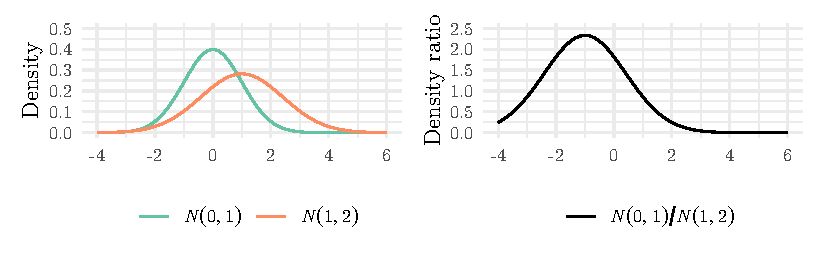
\includegraphics[width=1\textwidth,height=\textheight]{dr-utility-volker-kesteren_files/figure-pdf/fig-dr-plot-1.pdf}

}

\caption{\label{fig-dr-plot}Example of the density ratio of two normal
distributions with different means and variances (i.e., \(N(0,1)\) and
\(N(1,2)\)). Note that the density ratio is itself not a proper
density.}

\end{figure}

Over the past years, several methods for direct density ratio estimation
have been developed. Typically, these methods aim to minimize some
discrepancy \(\mathscr{D}(r(\boldsymbol{x}), \hat{r}(\boldsymbol{x}))\)
between the true density ratio and some density ratio model. One
commonly used discrepancy measure is the following squared error
\begin{equation}\protect\hypertarget{eq-squared-error}{}{
\mathcal{S}_0(r(\boldsymbol{x}), \hat{r}(\boldsymbol{x})) = 
\frac{1}{2} \int (\hat{r}(\boldsymbol{x}) - r(\boldsymbol{x}))^2 p_{obs}(\boldsymbol{x}) d\boldsymbol{x},
}\label{eq-squared-error}\end{equation} which can be considered as the
expected discrepancy between the two functions over the density of the
observed data. One could also use other discrepancy measures, such as
the binary or unnormalized Kullback-Leibler divergence or Basu's power
divergence (which are all members of the family of Bregman divergences;
for a detailed discussion, see
\protect\hyperlink{ref-sugiyama_bregman_2012}{Sugiyama, Suzuki, and
Kanamori 2012b}). It is convenient to model the density ratio with a
linear model, such that
\begin{equation}\protect\hypertarget{eq-dr-estimate}{}{
\hat{r}(\boldsymbol{x}) = \boldsymbol{\varphi}(\boldsymbol{x})\boldsymbol{\theta},
}\label{eq-dr-estimate}\end{equation} where
\(\boldsymbol{\varphi}(\boldsymbol{x})\) is a non-negative basis
function vector that transforms the data from a \(p\)-dimensional to a
\(b\)-dimensional space, and \(\boldsymbol{\theta}\) is a
\(b\)-dimensional parameter vector. Although the model is linear in its
parameters, the density ratio itself is a non-linear function of the
data if \(\boldsymbol{\varphi}(\boldsymbol{x})\) is a non-linear
transformation of the data, which it typically is.

To illustrate the idea of density ratio estimation, we briefly review
one method from the field: unconstrained least squares importance
fitting (\protect\hyperlink{ref-kanamori_ulsif_2009}{Kanamori, Hido, and
Sugiyama 2009}), which will also be used in our illustrations in the
upcoming section. The authors show that the squared error can be
rewritten as
\begin{equation}\protect\hypertarget{eq-sq-err-rewritten}{}{
\begin{aligned}
\mathcal{S}_0(r(\boldsymbol{x}), \hat{r}(\boldsymbol{x})) &=
\frac{1}{2}\int \hat{r}(\boldsymbol{x})^2p_{obs}(\boldsymbol{x}) d \boldsymbol{x} -
\int \hat{r}(\boldsymbol{x})r(\boldsymbol{x})p_{obs}(\boldsymbol{x})d\boldsymbol{x} + 
\frac{1}{2} \int r(\boldsymbol{x})^2 p_{obs}(\boldsymbol{x}) d\boldsymbol{x} \\
&= \frac{1}{2} \int \hat{r}(\boldsymbol{x})^2 p_{obs}(\boldsymbol{x}) d\boldsymbol{x} -
\int \hat{r}(\boldsymbol{x}) p_{syn}(\boldsymbol{x}) d \boldsymbol{x} + C,
\end{aligned}
}\label{eq-sq-err-rewritten}\end{equation} where \(r(\boldsymbol{x})\)
in the second term on the first line is rewritten in terms of the ratio
of \(p_{syn}(\boldsymbol{x})\) over \(p_{obs}(\boldsymbol{x})\). After
dropping the irrelevant (with respect to the data) constant \(C\), and
substituting the density ratio model as defined in
Equation~\ref{eq-dr-estimate}, we have
\begin{equation}\protect\hypertarget{eq-objective-int}{}{
\begin{aligned}
\mathcal{S}(r(\boldsymbol{x}), \hat{r}(\boldsymbol{x})) &=
\frac{1}{2} \int 
\boldsymbol{\theta}'
\boldsymbol{\varphi}(\boldsymbol{x})' 
\boldsymbol{\varphi}(\boldsymbol{x})
\boldsymbol{\theta}
p_{obs}(\boldsymbol{x}) 
d \boldsymbol{x}
- \int \boldsymbol{\varphi}(\boldsymbol{x}) \boldsymbol{\theta} p_{syn}(\boldsymbol{x}) d \boldsymbol{x}
\end{aligned}
}\label{eq-objective-int}\end{equation} as the objective function. The
integrals in Equation~\ref{eq-objective-int} are typically not
available, but can be replaced by empirical averages, such that
\begin{equation}\protect\hypertarget{eq-objective}{}{
\hat{\mathcal{S}}(r(\boldsymbol{x}), \hat{r}(\boldsymbol{x})) =
\frac{1}{2} \boldsymbol{\theta}' 
\Bigg(\frac{1}{n_{obs}}
\boldsymbol{\varphi}(\boldsymbol{x}_{obs})'\boldsymbol{\varphi}(\boldsymbol{x}_{obs})
\Bigg) \boldsymbol{\theta} -
\Bigg(
\frac{1}{n_{syn}} \boldsymbol{\varphi}(\boldsymbol{x}_{syn})' \boldsymbol{1}_{n_{syn}}
\Bigg)' \boldsymbol{\theta}.
}\label{eq-objective}\end{equation} It follows directly that the
parameter vector \(\boldsymbol{\theta}\) can be estimated as
\begin{equation}\protect\hypertarget{eq-param-est}{}{
\hat{\boldsymbol{\theta}} = \Big(
\frac{1}{n_{obs}}\boldsymbol{\varphi}(\boldsymbol{x}_{obs})'
\boldsymbol{\varphi}(\boldsymbol{x}_{obs})
\Big)^{-1} 
\Big(
\frac{1}{n_{syn}} \boldsymbol{\varphi}(\boldsymbol{x}_{syn})' \boldsymbol{1}_{n_{syn}}
\Big),
}\label{eq-param-est}\end{equation} which shows the least-squares nature
of the problem. Because one would expect the density ratio to be
non-negative, a non-negativity constraint for \(\boldsymbol{\theta}\)
can be added to the optimization problem, which would yield a convex
quadratic optimization problem that can be solved with dedicated
software. However, ignoring the non-negativity constraint has the
advantage that Equation~\ref{eq-objective} has an analytical expression,
which is numerically stable and computationally very efficient. The
corresponding downside of having negative estimated density ratio values
can be remedied by setting negative values in
\(\hat{\boldsymbol{\theta}}\) to \(0\).

From here, we are left with two remaining tasks. First, one typically
wants to add a regularization parameter \(\lambda\) to the objective
function to prevent overfitting and ensure positive-definiteness. In the
unconstrained realm, a ridge penalty
\((\lambda/2) \boldsymbol{\theta}'\boldsymbol{\theta}\) is typically
added to the optimization problem in Equation~\ref{eq-objective}. Adding
this to the solution in Equation~\ref{eq-param-est} yields
\begin{equation}\protect\hypertarget{eq-param-est-reg}{}{
\hat{\boldsymbol{\theta}} = \Big(
\frac{1}{n_{obs}}\boldsymbol{\varphi}(\boldsymbol{x}_{obs})'
\boldsymbol{\varphi}(\boldsymbol{x}_{obs})
+ \lambda \boldsymbol{I}_b
\Big)^{-1} 
\Big(
\frac{1}{n_{syn}} \boldsymbol{\varphi}(\boldsymbol{x}_{syn})' \boldsymbol{1}_{n_{syn}}
\Big),
}\label{eq-param-est-reg}\end{equation} where \(\boldsymbol{I}_b\)
denotes a \(b \times b\) identity matrix. The regularization parameter
\(\lambda\) can be chosen via cross-validation. Conveniently, the
\emph{leave-one-out cross-validation} score can also be computed
analytically when using unconstrained least-squares importance fitting
(see Section 3.4 in
\protect\hyperlink{ref-kanamori_ulsif_2009}{Kanamori, Hido, and Sugiyama
2009}). Second, we need to specify the basis functions used in the
density ratio model. A common choice is to use a Gaussian kernel, which
quantifies the similarity between observations as
\begin{equation}\protect\hypertarget{eq-gauss-kernel}{}{
\boldsymbol{\varphi}(\boldsymbol{x}) = 
\boldsymbol{K}(\boldsymbol{x}, \boldsymbol{c}) = 
\exp \Bigg(-\frac{\lVert \boldsymbol{x} - \boldsymbol{c}\rVert^2}{2\sigma^2} \Bigg),
}\label{eq-gauss-kernel}\end{equation} where \(\boldsymbol{c}\) denotes
the Gaussian centers and \(\sigma\) controls the kernel width. The
bandwidth parameter \(\sigma\) can also be selected using
cross-validation. Typically a subset of the numerator samples are chosen
as the Gaussian centers, because the density ratio tends to take large
values at locations where the numerator density has more mass than the
denominator density. To estimate the density ratio accurately, we may
use many kernels where the density ratio is expected to be large,
whereas having few kernels might suffice in the locations where the
density ratio is small. Hence, we place many kernels where the synthetic
data density is large, by taking a sample of the synthetic records as
Gaussian centers, with the number of samples \(n_c\) dependent on the
computational resources available (but typically
\(\min(100, n_{syn}) \leq n_{c} \leq \min(1000, n_{syn})\)).

After estimating the density ratio, one can assess whether the numerator
and denominator densities differ significantly via a permutation test.
To this end, Sugiyama, Suzuki, et al.
(\protect\hyperlink{ref-sugiyama_lstst_2011}{2011}) propose a two-sample
test that quantifies the discrepancy between the numerator (synthetic)
and denominator (observed) samples through the density ratio, using the
Pearson divergence
\(\mathcal{P}(p_{syn}(\boldsymbol{x}), p_{obs}(\boldsymbol{x}))\) as a
test statistic: \begin{equation}\protect\hypertarget{eq-pearson-test}{}{
\hat{\mathcal{P}}(p_{syn}(\boldsymbol{x}), p_{obs}(\boldsymbol{x}))
= \frac{1}{2n_{syn}} \sum^{n_{syn}}_{i=1} \hat{r}(\boldsymbol{x}_{syn}^{(i)}) -
\frac{1}{n_{obs}} \sum^{n_{obs}}_{j=1} \hat{r}(\boldsymbol{x}_{obs}^{(j)}) + \frac{1}{2}.
}\label{eq-pearson-test}\end{equation} Intuitively, this discrepancy
captures how different the synthetic data is from the observed data by
measuring the distance from the density ratio at the observed data
points to the density ratio at the synthetic data points. As we show in
our empirical examples, this statistic is difficult to interpret in an
absolute sense. However, we show that it is useful as a relative measure
of fit of the different synthetic data sets. Additionally, the value of
the test statistic can be used to construct a hypothesis test for the
lack of fit of the synthetic data using a permutation test. An empirical
\(p\)-value can then be calculated as the proportion of test statistics
under the null model that are greater than the observed test statistic.
In this way, it can be assessed whether the synthetic data model is
misspecified, by comparing the observed value to what can be expected
under a correctly specified synthesis model.

\hypertarget{density-ratio-estimation-as-a-utility-measure-simulated-and-empirical-examples}{%
\section{Density ratio estimation as a utility measure: Simulated and
empirical
examples}\label{density-ratio-estimation-as-a-utility-measure-simulated-and-empirical-examples}}

In this section, we illustrate density ratio estimation using
unconstrained least-squares importance fitting. In a small simulation,
we show that the method gives reasonable results when the goal is to
estimate a density ratio in several parametric examples. Subsequently,
we use these examples to show how the results of density ratio
estimation can be used as a measure of utility, and we describe how a
lack of fit of the synthesis model can be inferred from the density
ratio. Starting with univariate examples, we compare the density ratio
two-sample test with existing goodness-of-fit measures (the
Kolmogorov-Smirnov test and the \(pMSE\)). As a final illustration, we
build upon the work by Drechsler
(\protect\hyperlink{ref-drechsler_utility_2022}{2022}), and showcase how
density ratio estimation improves upon utility assessment through the
\(pMSE\) in a multivariate example. All analyses were conducted in
\texttt{R} (Version 4.3.0; \protect\hyperlink{ref-R}{R Core Team 2023}),
and the code is available on
\href{https://github.com/thomvolker/unece-density-ratio}{GitHub}. The
software used to perform density ratio estimation is implemented in an
\texttt{R}-package called \texttt{densityratio}
(\protect\hyperlink{ref-densityratio}{Volker 2023}).

\hypertarget{density-ratio-estimation-in-simulated-univariate-examples}{%
\subsection{Density ratio estimation in simulated univariate
examples}\label{density-ratio-estimation-in-simulated-univariate-examples}}

To provide an intuition about the performance of unconstrained
least-squares importance fitting, we apply it to a simplified example of
a typical situation in the synthetic data field. When creating synthetic
data, we often have a complex, usually unknown, data distribution that
we want to approximate with a model. We generally lack information to
correctly model real-world phenomena, and even if we would have
sufficient information, some important factors might be missing from the
data, or the model might be so complex that it is unfeasible to actually
simulate data from it. For the sake of illustrational clarity, we
generate univariate data according to four true data-generating
mechanisms:

\begin{enumerate}
\def\labelenumi{\arabic{enumi}.}
\tightlist
\item
  \(\text{Laplace}(\mu = 1, b = 1)\)
\item
  \(\text{Log-normal}(\mu_{\log} = \log{\{\mu^2/\sqrt{\mu^2 + \sigma^2_x}\}}, \sigma^2_{\log} = \log{\{1 + \sigma^2_x/\mu^2\}})\),
  with \(\mu = 1\) and \(\sigma^2_x = 2\)
\item
  Location-scale \(t\)-distribution
  \(lst(\mu = 1, \tau^2 = 1, \nu = 4)\)
\item
  \(\text{Normal}(\mu = 1, \sigma^2_x = 2)\)
\end{enumerate}

Note that these four distributions all have the same population mean
\(\mu = 1\) and the same population variance \(\sigma^2_x = 2\). From
each distribution, we generate \(200\) data sets of size
\(n_{obs} = 250\). For all scenarios, we approximate the true
data-generating mechanism by drawing \(200\) data sets of size
\(n_{syn} = 250\) from a normal distribution
(\(\text{Normal}(\mu = 1, \sigma^2_x = 2)\)), such that we accurately
model the mean and variance of each true data-generating distribution
(see also Figure~\ref{fig-densities} for a graphical depiction of the
true and synthetic data densities). Note that in the fourth scenario, we
thus model the true data-generating distribution correctly, which is
included to get some intuition on how density ratio estimation performs
when we specify the synthesis model correctly. All density ratios were
estimated with the exact same model specifications: we used \(100\)
observations from the synthetic data as Gaussian centers and performed
cross-validation over \(10\) values of the Gaussian kernel width
\(\sigma\) and \(10\) values of the regularization parameter
\(\lambda\).

\begin{figure}[t]

{\centering 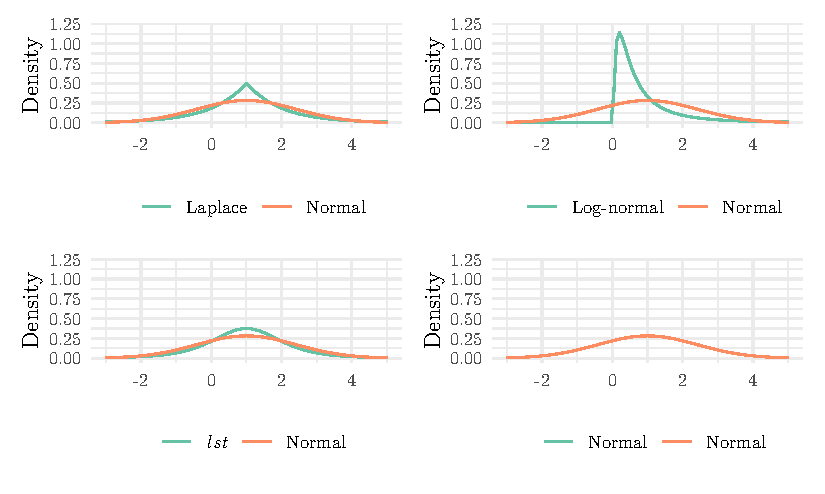
\includegraphics[width=1\textwidth,height=\textheight]{dr-utility-volker-kesteren_files/figure-pdf/fig-densities-1.pdf}

}

\caption{\label{fig-densities}True and synthetic data densities for the
examples considered (Laplace, Log-normal, \(t\) and Normal), all
distributions have mean \(\mu = 1\) and variance \(\sigma^2_x = 2\).
Note that the true and synthetic data density in the bottom right plot
are completely overlapping.}

\end{figure}

\begin{figure}[t]

{\centering 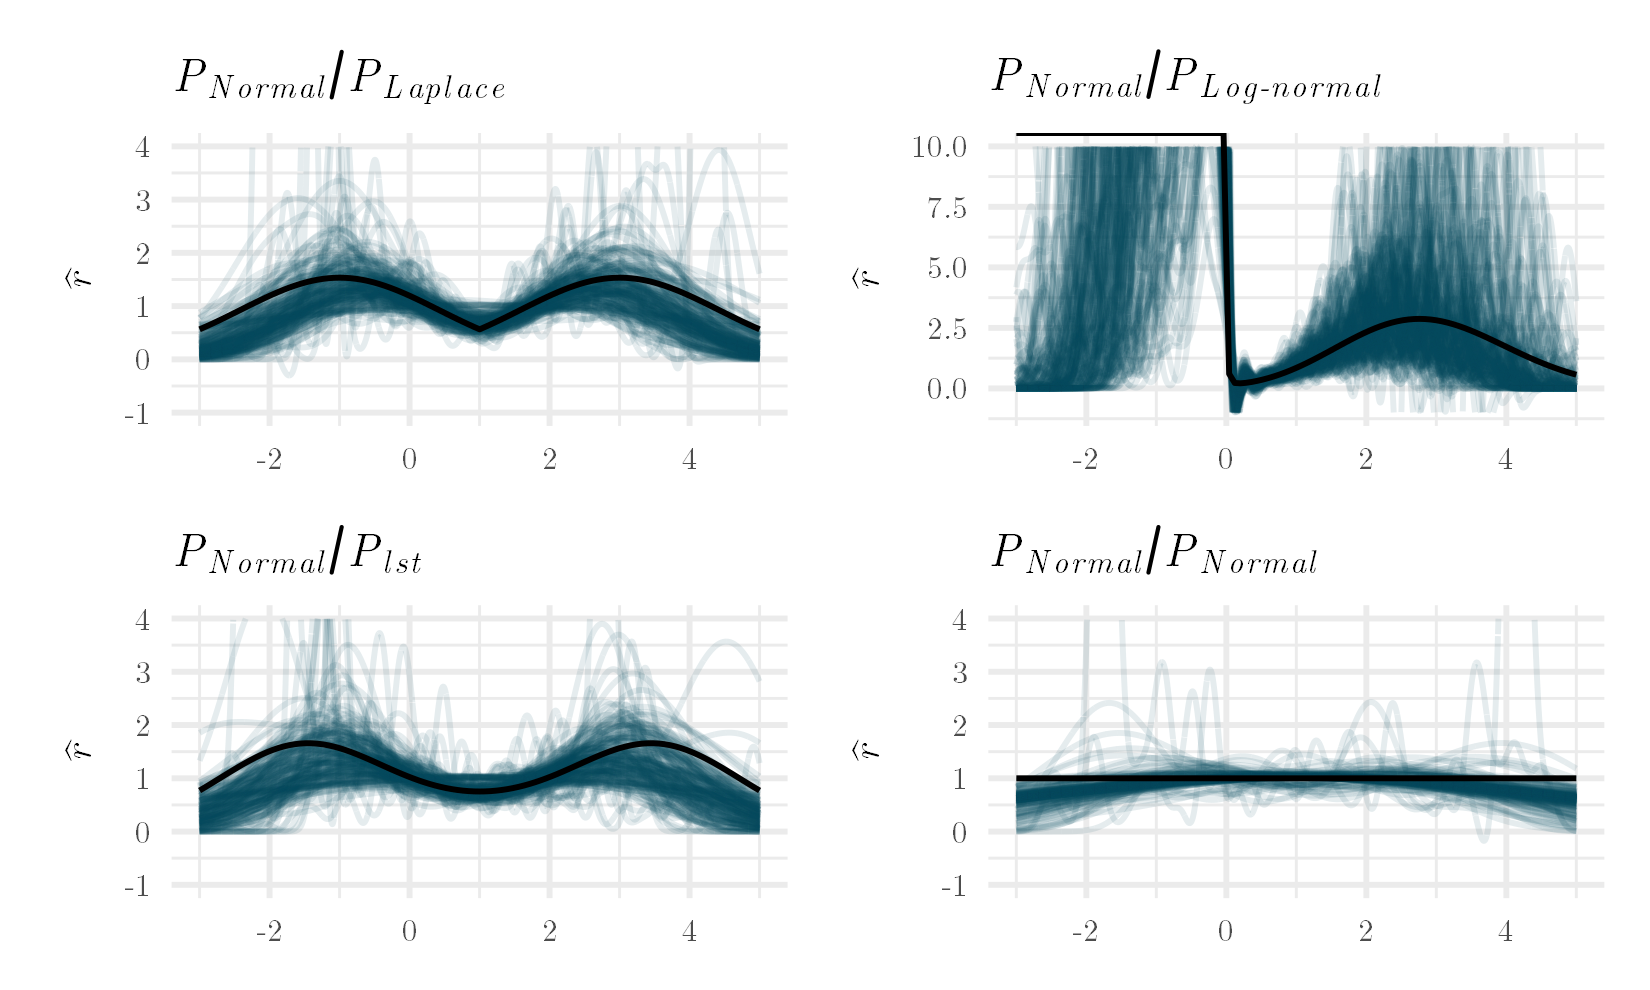
\includegraphics[width=1\textwidth,height=\textheight]{dr-utility-volker-kesteren_files/figure-pdf/fig-sim-dr-1.png}

}

\caption{\label{fig-sim-dr}Estimated density ratios by unconstrained
least-squares importance fitting in four univariate examples: A Laplace
distribution, a log-normal distribution, a \(t\)-distribution and a
normal distribution, all approximated by a normal distribution with the
same mean and variance as the original distributions.}

\end{figure}

Figure~\ref{fig-sim-dr} shows how the estimated density ratios for the
\(200\) simulated datasets in each scenario (the blue lines in each
subfigure) compared to the true density ratios (the black lines). In
each of the four figures, the estimated density ratios follow the
general trend of the true density ratios. In the top-left plot, showing
the ratio of the normal distribution over the Laplace distribution, the
density ratio decreases at the sides, then increases when moving towards
the center, but decreases again close to the center. The same can be
observed in the bottom-left plot, which shows the normal distribution
over the \(lst\)-distribution. In the top right panel, the estimated
density ratios are typically large for negative values, very close to
zero (or even negative) around the peak of the log-normal distribution,
and subsequently increasing and later on decreasing again. In the bottom
right panel, where both distributions are identical, the majority of the
estimated density ratios are very flat, tending towards zero to some
extent at the edges of the figure where only few data points are
located. Moreover, all figures show some highly variable estimated
density ratios due to modest overfitting regardless of the
cross-validation scheme, whereas the normal versus log-normal figure
shows many highly variable estimates outside of the center of the
figure, due to the fact that either the synthetic or the observed data
has only few cases in these regions. Normally, the stability of the
estimates increases with the sample size. Figure~\ref{fig-sim-dr} also
shows one of the main advantages of density ratio estimation as a
utility measure, in the sense that it provides a quantification of the
fit for every data point. At those locations where the estimated density
ratio takes large values, there are too many synthetic observations
compared to what should be expected based on the observed data, whereas
at the points where the density ratio is close to zero, there are too
few synthetic observations relative to the observed data. Likewise, a
high density ratio value for a synthetic record indicates that this
point deviates from what would be typical under the observed
data-generating mechanism.

As it is hard to infer from visualizations whether the misfit could
arise from chance alone, or whether the synthetic data model is
misspecified, we formally evaluate the fit of the synthetic data by
performing statistical inference using the Pearson divergence as a
measure of discrepancy (see Equation~\ref{eq-pearson-test}). To explore
the properties of the corresponding permutation test, we compare it in
terms of power and Type I error rate with the Kolmogorov-Smirnov test
and with a \(pMSE\)-based test, obtained by performing a permutation
test and assessing the proportion of times the permuted \(pMSE\)s are
larger than the observed \(pMSE\)
(\protect\hyperlink{ref-snoke_utility_2018}{Snoke et al. 2018}). The
\(pMSE\)s are calculated by using the \texttt{utility.tab()} function
with default settings from the \texttt{R}-package \texttt{synthpop}
(\protect\hyperlink{ref-nowok2016}{Nowok, Raab, and Dibben 2016}).
Table~\ref{tbl-test-pvals} shows that in terms of evaluating the misfit
of the synthetic data, the density ratio-based test has statistical
power similar to the \(pMSE\)-based test. That is, when the synthetic
data model differs from the observed data-generating mechanism, the
density ratio-based test and the \(pMSE\)-based test indicate
significant misfit in approximately \(60\%\) of the simulations for the
Laplace data, \(100\%\) for the log-normal data and \(50\%\) for the
location-scale \(t\)-distributed data. Both methods achieve considerably
higher power than the Kolmogorov-Smirnov test. When the synthesis model
is correctly specified, all three methods achieve a nominal Type I error
rate close to \(0.05\).

\hypertarget{tbl-test-pvals}{}
\begin{table}
\caption{\label{tbl-test-pvals}Proportion of significant tests for the fit of the synthetic data. }\tabularnewline

\centering
\begin{tabular}[t]{lrrr}
\toprule
Data & Density ratio & Kolmogorov-Smirnov & $pMSE$\\
\midrule
Laplace & 0.620 & 0.375 & 0.610\\
Log-normal & 1.000 & 1.000 & 1.000\\
$lst$ & 0.495 & 0.235 & 0.495\\
Normal & 0.050 & 0.045 & 0.040\\
\bottomrule
\end{tabular}
\end{table}

\hypertarget{density-ratio-estimation-for-synthetic-current-population-survey-data}{%
\subsection{Density ratio estimation for synthetic Current Population
Survey
data}\label{density-ratio-estimation-for-synthetic-current-population-survey-data}}

To evaluate the properties of density ratio estimation in a real-life
example, we repeat Drechsler's
(\protect\hyperlink{ref-drechsler_utility_2022}{2022}) illustration of
the \(pMSE\) as a fit-for-purpose and global utility measure with a
subset of the March 2000 U.S. Current Population Survey, but now using
density ratio estimation. Notably, we use the exact same (default)
density ratio model specifications as in the previous simulations, both
for evaluating the utility of the variables separately and over the
synthetic data sets as a whole. We use exactly the same data as
Drechsler (\protect\hyperlink{ref-drechsler_utility_2022}{2022}), that
is, the variables \emph{Sex}, \emph{Race}, \emph{Marital Status},
\emph{Highest attained education level}, \emph{Age}, \emph{Social
security payments}, \emph{Household property taxes} and \emph{Household
income}, measured on \(n = 5000\) individuals (descriptive statistics
are provided in Table~\ref{tbl-desc} and a graphical depiction of the
numeric variables is shown in Figure~\ref{fig-vars-orig}, both in
Appendix A). Note that the continuous variables are typically
non-normal, while the variables \emph{Household property taxes} and
\emph{Social security payments} in addition have a point-mass at zero.
Data synthesis is done using the \texttt{R}-package \texttt{synthpop}
(\protect\hyperlink{ref-nowok2016}{Nowok, Raab, and Dibben 2016}), using
the same synthesis strategies as used in Drechsler
(\protect\hyperlink{ref-drechsler_utility_2022}{2022}). We thus refer to
this paper for details about the synthesis strategies, and only briefly
describe the synthesis models here. Three of the synthetic data sets are
created using parametric models: \emph{Sex} and \emph{Race} are
synthesized with logistic regression models, \emph{Marital status} and
\emph{Highest attained education} are synthesized using multinomial
regression, and all continuous variables are synthesized using a linear
model. The parametric synthesis models build up in complexity in how
they model the continuous variables in the following way: the first
model (labelled \emph{naive}) does not take the distributions of the
variables into account, and models the variables on the original scale;
the second model (called \emph{transformed}) transforms the variables by
taking their cubic root and subsequently applies a linear model to the
transformed variables; the third model (labelled \emph{semi-continuous})
also transforms all variables to the cubic root scale, but in addition
separately models the point mass at zero for the variables
\emph{Household property taxes} and \emph{Social security payments}
separately, after which a linear model is used for the non-zero values.
The non-parametric synthesis model applies classification and regression
trees (CART) to all variables, augmented by smoothing through kernel
density estimation in the terminal nodes. For all strategies, \(m = 5\)
synthetic data sets are generated, and the utility is assessed by
averaging the Pearson divergence over those sets. As noted by Drechsler
(\protect\hyperlink{ref-drechsler_utility_2022}{2022}), based on the
sequential refinements of the parametric synthesis models, one would
expect the utility to improve with every parametric model, leaving open
how the CART models compare to the parametric models.

\begin{figure}[t]

{\centering 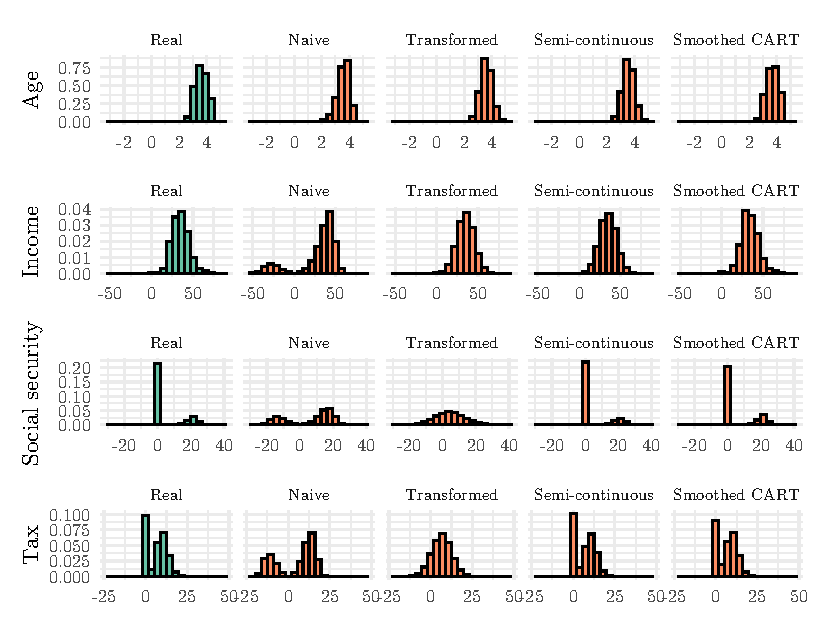
\includegraphics[width=1\textwidth,height=\textheight]{dr-utility-volker-kesteren_files/figure-pdf/fig-syn-dist-1.pdf}

}

\caption{\label{fig-syn-dist}Real and synthetic data distributions for
the variables age, household income (income), household property taxes
(tax) and social security payments (social security) on a cubic root
scale (using \(f(x) = \text{sign}(x)|x|^{1/3}\)).}

\end{figure}

Figure~\ref{fig-syn-dist} shows how the increasing complexity of the
synthesis models leads to increasingly realistic synthetic data
distributions (all variables are plotted on a cubic root scale using
\(f(x) = \text{sign}(x)|x|^{1/3}\) to also allow for negative values).
It is evident that the \emph{naive} synthesis strategy does a poor job
for all variables except \emph{Age}, whereas the \emph{transformed}
strategy does a poor job for \emph{Tax} and \emph{Social security}. The
\emph{semi-continuous} strategy seems to fit well for all variables,
similarly to the data created with CART, although the latter method
preserves the non-normality of the non-zero values in \emph{Social
security} slightly better. The insights from visual inspection are
entirely corroborated by the relative Pearson divergences as given by
density ratio estimation (see Figure~\ref{fig-PE-div}). For all
variables, the \emph{naive} synthesis method performs worst. Typically,
the \emph{transformed} synthesis improves the synthetic data to some
extent, although the difference is relatively small for \emph{Age},
because here the \emph{naive} synthesis strategy already performed
reasonable. For both \emph{Age} and \emph{Income}, the
\emph{transformed} strategy performs similarly to both the
\emph{semi-continuous} and the CART strategies, because for these
variables there is no point-mass to model separately. For the variables
where a point-mass is modeled separately (e.g., \emph{Social security}
and \emph{Tax}), the \emph{semi-continuous} approach clearly outperforms
the \emph{transformed} strategy. Lastly, CART outperforms the
\emph{naive} and \emph{transformed} strategies, and performs highly
similar to the \emph{semi-continuous} approach.

When modelling the density ratio over all variables in the data
simultaneously (including the categorical variables, for simplicity
recoded as numeric variables to be included in density ratio
estimation), we see the same picture emerging. Figure~\ref{fig-PE-div}
shows the stepwise improvements in utility when refining the synthesis
models. \emph{Naive} synthesis clearly performs worst, followed by the
\emph{transformed} strategy. Both strategies are outperformed by the
\emph{semi-continuous} approach, which performs more or less on par with
CART. These results compare favorably with utility assessment through
the \(pMSE\) as reported in Drechsler
(\protect\hyperlink{ref-drechsler_utility_2022}{2022}). The evaluation
of utility through the \(pMSE\) shows no improvement when going from
\emph{naive} to \emph{transformed} synthesis, whereas some \(pMSE\)
models qualified the \emph{naive} approach as better than the
\emph{transformed} approach. The improvement from the first two
strategies to \emph{semi-continuous} and CART was picked up by most
\(pMSE\) models. Hence, the utility assigned by density ratio estimation
was more in line with the refinements to the synthesis models than the
utility scores that were obtained with the \(pMSE\).

\begin{figure}[t]

{\centering 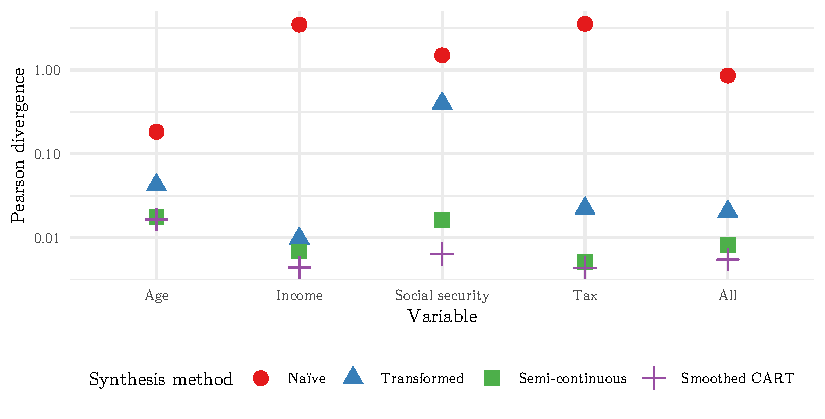
\includegraphics[width=1\textwidth,height=\textheight]{dr-utility-volker-kesteren_files/figure-pdf/fig-PE-div-1.pdf}

}

\caption{\label{fig-PE-div}Pearson divergence estimates after different
synthesis strategies for the separate variables and the synthetic data
sets as a whole.}

\end{figure}

\hypertarget{discussion}{%
\section{Discussion}\label{discussion}}

When creating synthetic data with the goal of private data release, it
is crucial to evaluate its quality. This allows the data provider to
decide whether the synthetic data is useful for the purposes of the
release or requires further refinements, and to inform the data user
about the analyses that can be reliably conducted. In this paper, we
showed that density ratio estimation provides a promising framework to
evaluate the utility of synthetic data and we implemented the approach
in the R-package \texttt{densityratio}
(\protect\hyperlink{ref-densityratio}{Volker 2023}). In a small
simulation, we showed that for sample sizes as small as \(250\)
observations, it was possible to obtain a rather accurate estimate of
the true density ratio. Moreover, in terms of statistical power, density
ratio estimation performed on par with the \(pMSE\) and outperforms the
Kolmogorov-Smirnov test in the univariate comparisons considered. When
evaluating density ratio estimation on multiple synthetic versions of a
real-world data set, we showed that the method was able to pick up all
improvements in the synthesis models made, in contrast to the \(pMSE\)
(as shown by \protect\hyperlink{ref-drechsler_utility_2022}{Drechsler
2022}). Moreover, whereas Drechsler
(\protect\hyperlink{ref-drechsler_utility_2022}{2022}) showed that
quantification of the utility through the \(pMSE\) was highly dependent
on the propensity score model, density ratio estimation possesses
automatic model selection in terms of its hyperparameters, and thus
requires almost no user-specification. We emphasize that we used the
same default settings for our simulations and for modelling all
individual variables and the entire data sets in our empirical example,
regardless of the varying scales of the variables and other
variable-specific peculiarities, such as point masses and non-normality.

Although this paper focused on various comparisons, we note that there
are many connections between density ratio estimation and existing
utility measures. For example, the \(pMSE\) can be considered as an
instance of density ratio estimation, in which the propensity scores are
used to model the density ratio. Specifically, the propensity scores can
be transformed into the posterior odds of any record belonging to the
synthetic data versus the observed data, which yields an estimate of the
density ratio. Additionally, Sugiyama, Suzuki, and Kanamori
(\protect\hyperlink{ref-sugiyama_suzuki_kanamori_2012}{2012a}) show that
density ratio estimation can be regarded as divergence estimation
between the numerator and denominator density. As such, the framework
also encompasses estimation of, for example, the Kullback-Leibler
divergence, proposed as utility measure by Karr et al.
(\protect\hyperlink{ref-karr_utility_2006}{2006}). Lastly, density ratio
estimation can be seen as an extension of the ``ratio of estimates''
utility measure (\protect\hyperlink{ref-taub2020}{Taub, Elliot, and
Sakshaug 2020}), which is defined for categorical data as the ratio of
observed and synthetic frequencies (scaled to be between \(0\) and \(1\)
by putting the largest count in the denominator), to continuous data. As
such, the density ratio framework encapsulates various measures to
evaluate the utility of synthetic data.

Expanding upon the appealing properties discussed in this paper, we
foresee three additional advantages of the density ratio framework.
\textbf{(1) Utility on the level of individual data points.} The density
ratio is estimated over the entire (multivariate) space of the data, and
these estimates can be used to quantify the deviation of every synthetic
data point with respect to the observed data. These values can help to
identify sub-spaces that are poorly reproduced in the synthetic data,
but they might also yield additional benefits. On a low level, these
values might be used to discard observations that are considered as
being too far from the observed data to be realistic, or resample
observations that are typical in the observed data but occur
infrequently in the synthetic data. On a higher level, one could
potentially use density ratio values to reweigh analyses with synthetic
data to bring the results closer to the real data. Future research
should evaluate the merits of this approach, but also potential privacy
risks of disseminating such weights. \textbf{(2) Density ratios for
specific utility.} Another potential benefit is that the use of the
method is not necessarily restricted to the level of the data at hand.
Density ratio estimation could give rise to analysis-specific utility
measures by applying the framework on the posterior distributions of
parameters (or an approximation hereof). That is, if the distribution of
the parameters of the analysis model can be approximated, for example by
a multivariate normal distribution, or when samples from the parameter
distribution are available, it is possible to either analytically
calculate the density ratio, or estimate it using the techniques
described above. The resulting density ratio can then again be used to
quantify how similar the distributions are. \textbf{(3) Extensions to
high-dimensional data.} When the number of variables grows large
relative to the number of observations, direct density ratio estimation
through unconstrained least-squares importance fitting might become
inaccurate. However, the density ratio estimation framework possesses
readily available extensions that include dimension reduction as part of
the estimation process, which yields the advantage of simultaneously
optimizing the density ratio solution with the dimension-reduced
subspace of the data
(\protect\hyperlink{ref-sugiyama_lhss_2011}{Sugiyama, Yamada, et al.
2011}).

Finally, let us remark that there are several open questions that need
to be addressed before density ratio estimation can be fully
incorporated in synthetic data evaluation pipelines. First,
methodological research should investigate how to deal with categorical
variables. In the density ratio estimation framework, the focus has
almost exclusively been on numeric data, whereas in practical
situations, categorical data is all too common. In this paper, we dealt
with the issue by simply transforming the categorical variables into
numeric variables, but other techniques might yield more accurate
results. To name three other strategies, one could transform the
categorical variables into dummy variables, use a different distance
metric that allows for categorical data when specifying the kernel, or
assume an underlying continuous latent space, and model the categorical
variables on this space. Second, which default settings to use in
density ratio estimation is still an open question. Although we showed
that our default settings performed reasonably, most choices lack a
strong theoretical justification. Potentially, the utility of synthetic
data can be evaluated much more accurately by, for example, choosing a
different kernel, choosing the centers in the Gaussian kernel in a
different way, or using a broader range of bandwidth and regularization
parameters. Lastly, it must be evaluated what information from density
ratio estimation can be released to the public without incurring severe
privacy risks. Presumably, releasing the Pearson divergence, potentially
augmented with a \(p\)-value to indicate the lack of fit of the
synthetic data, will yield only little additional privacy risk. However,
releasing visualizations of the estimated density ratio or the estimated
density ratio values themselves might cause unacceptable threats,
especially for observations in the tails of the distribution. Future
research can make efforts to privatize the output from density ratio
estimation, or at least investigate what risks are related to releasing
the output of the estimation process. With these promising avenues for
extensions in mind, we conclude that the density ratio estimation
framework provides a viable and intuitive alternative to existing
utility measures that can enhance synthetic data workflows.

\hypertarget{acknowledgements}{%
\section{Acknowledgements}\label{acknowledgements}}

We are grateful to Dr.~Jörg Drechsler for sharing his cleaned version of
the Current Population Survey data and the corresponding analysis code.

\hypertarget{references}{%
\section{References}\label{references}}

\hypertarget{refs}{}
\begin{CSLReferences}{1}{0}
\leavevmode\vadjust pre{\hypertarget{ref-SIPP_Beta_2006}{}}%
Abowd, John M., Martha Stinson, and Gary Benedetto. 2006. {``Final
Report to the Social Security Administration on the {SIPP/SSA/IRS}
Public Use File Project.''} Longitudinal Employer-Household Dynamics
Program, U.S. Bureau of the Census, Washington, DC.
\url{https://ecommons.cornell.edu/bitstream/handle/1813/43929/SSAfinal.pdf?sequence=3\&isAllowed=y}.

\leavevmode\vadjust pre{\hypertarget{ref-drechsler2012}{}}%
Drechsler, Jörg. 2012. {``New Data Dissemination Approaches in Old
Europe {\textendash} Synthetic Datasets for a German Establishment
Survey.''} \emph{Journal of Applied Statistics} 39 (2): 243--65.
\url{https://doi.org/10.1080/02664763.2011.584523}.

\leavevmode\vadjust pre{\hypertarget{ref-drechsler_utility_2022}{}}%
---------. 2022. {``Challenges in Measuring Utility for Fully Synthetic
Data.''} In \emph{Privacy in Statistical Databases}, edited by Josep
Domingo-Ferrer and Maryline Laurent, 220--33. Cham: Springer
International Publishing.
\url{https://doi.org/10.1007/978-3-031-13945-1_16}.

\leavevmode\vadjust pre{\hypertarget{ref-drechsler2023}{}}%
Drechsler, Jörg, and Anna-Carolina Haensch. 2023. {``30 Years of
Synthetic Data.''} \url{https://doi.org/10.48550/ARXIV.2304.02107}.

\leavevmode\vadjust pre{\hypertarget{ref-dwork_dp_2006}{}}%
Dwork, Cynthia. 2006. {``Differential Privacy.''} In \emph{Automata,
Languages and Programming}, edited by Michele Bugliesi, Bart Preneel,
Vladimiro Sassone, and Ingo Wegener, 1--12. Berlin, Heidelberg: Springer
Berlin Heidelberg. \url{https://doi.org/10.1007/11787006_1}.

\leavevmode\vadjust pre{\hypertarget{ref-hawala_synthetic_2008}{}}%
Hawala, Sam. 2008. \emph{Producing Partially Synthetic Data to Avoid
Disclosure}.
\url{http://www.asasrms.org/Proceedings/y2008/Files/301018.pdf}.

\leavevmode\vadjust pre{\hypertarget{ref-shohei_dre_outlier_2008}{}}%
Hido, Shohei, Yuta Tsuboi, Hisashi Kashima, Masashi Sugiyama, and
Takafumi Kanamori. 2008. {``Inlier-Based Outlier Detection via Direct
Density Ratio Estimation.''} In \emph{2008 Eighth IEEE International
Conference on Data Mining}, edited by Fosca Giannotti, Dimitrios
Gunopulos, Franco Turini, Carlo Zaniolo, Naren Ramakrishnan, and Xindong
Wu, 223--32. \url{https://doi.org/10.1109/ICDM.2008.49}.

\leavevmode\vadjust pre{\hypertarget{ref-hu2019}{}}%
Hu, Jingchen. 2019. {``Bayesian Estimation of Attribute and
Identification Disclosure Risks in Synthetic Data.''} \emph{Transactions
on Data Privacy} 12: 61--89.
\url{http://www.tdp.cat/issues16/tdp.a313a18.pdf}.

\leavevmode\vadjust pre{\hypertarget{ref-jordon2018pategan}{}}%
Jordon, James, Jinsung Yoon, and Mihaela van der Schaar. 2019.
{``{PATE}-{GAN}: Generating Synthetic Data with Differential Privacy
Guarantees.''} In \emph{International Conference on Learning
Representations}. \url{https://openreview.net/forum?id=S1zk9iRqF7}.

\leavevmode\vadjust pre{\hypertarget{ref-kanamori_ulsif_2009}{}}%
Kanamori, Takafumi, Shohei Hido, and Masashi Sugiyama. 2009. {``A
Least-Squares Approach to Direct Importance Estimation.''} \emph{Journal
of Machine Learning Research} 10 (48): 1391--1445.
\url{http://jmlr.org/papers/v10/kanamori09a.html}.

\leavevmode\vadjust pre{\hypertarget{ref-Kanamori2012}{}}%
Kanamori, Takafumi, Taiji Suzuki, and Masashi Sugiyama. 2012.
{``Statistical Analysis of Kernel-Based Least-Squares Density-Ratio
Estimation.''} \emph{Machine Learning} 86 (3): 335--67.
\url{https://doi.org/10.1007/s10994-011-5266-3}.

\leavevmode\vadjust pre{\hypertarget{ref-karr_utility_2006}{}}%
Karr, Alan F., Christine N. Kohnen, Anna Oganian, Jerome P. Reiter, and
Ashish P. Sanil. 2006. {``A Framework for Evaluating the Utility of Data
Altered to Protect Confidentiality.''} \emph{The American Statistician}
60 (3): 224--32. \url{https://doi.org/10.1198/000313006X124640}.

\leavevmode\vadjust pre{\hypertarget{ref-little_statistical_1993}{}}%
Little, Roderick J. A. 1993. {``Statistical Analysis of Masked Data.''}
\emph{Journal of Official Statistics} 9 (2): 407--7.
\url{https://www.scb.se/contentassets/ca21efb41fee47d293bbee5bf7be7fb3/statistical-analysis-of-masked-data.pdf}.

\leavevmode\vadjust pre{\hypertarget{ref-liu_change_2013}{}}%
Liu, Song, Makoto Yamada, Nigel Collier, and Masashi Sugiyama. 2013.
{``Change-Point Detection in Time-Series Data by Relative Density-Ratio
Estimation.''} \emph{Neural Networks} 43: 72--83.
\url{https://doi.org/10.1016/j.neunet.2013.01.012}.

\leavevmode\vadjust pre{\hypertarget{ref-mcclure2016assessing}{}}%
McClure, David, and Jerome P Reiter. 2016. {``Assessing Disclosure Risks
for Synthetic Data with Arbitrary Intruder Knowledge.''}
\emph{Statistical Journal of the IAOS} 32 (1): 109--26.
\url{https://doi.org/10.3233/SJI-160957}.

\leavevmode\vadjust pre{\hypertarget{ref-nikolenko2021}{}}%
Nikolenko, Sergey I. 2021. \emph{Synthetic Data for Deep Learning}.
Springer International Publishing.
\url{https://doi.org/10.1007/978-3-030-75178-4}.

\leavevmode\vadjust pre{\hypertarget{ref-nowok2016}{}}%
Nowok, Beata, Gillian M. Raab, and Chris Dibben. 2016.
{``{\emph{Synthpop}:} Bespoke Creation of Synthetic Data in
{\emph{R}}.''} \emph{Journal of Statistical Software} 74 (11).
\url{https://doi.org/10.18637/jss.v074.i11}.

\leavevmode\vadjust pre{\hypertarget{ref-obermeyer2019}{}}%
Obermeyer, Ziad, Brian Powers, Christine Vogeli, and Sendhil
Mullainathan. 2019. {``Dissecting Racial Bias in an Algorithm Used to
Manage the Health of Populations.''} \emph{Science} 366 (6464): 447--53.
\url{https://doi.org/10.1126/science.aax2342}.

\leavevmode\vadjust pre{\hypertarget{ref-patki2016}{}}%
Patki, Neha, Roy Wedge, and Kalyan Veeramachaneni. 2016. {``The
Synthetic Data Vault.''} \emph{2016 IEEE International Conference on
Data Science and Advanced Analytics (DSAA)}, October.
\url{https://doi.org/10.1109/dsaa.2016.49}.

\leavevmode\vadjust pre{\hypertarget{ref-R}{}}%
R Core Team. 2023. \emph{R: A Language and Environment for Statistical
Computing}. Vienna, Austria: R Foundation for Statistical Computing.
\url{https://www.R-project.org/}.

\leavevmode\vadjust pre{\hypertarget{ref-Reiter_Mitra_2009}{}}%
Reiter, Jerome P., and Robin Mitra. 2009. {``Estimating Risks of
Identification Disclosure in Partially Synthetic Data.''} \emph{Journal
of Privacy and Confidentiality} 1 (1).
\url{https://doi.org/10.29012/jpc.v1i1.567}.

\leavevmode\vadjust pre{\hypertarget{ref-rosenbaum_propensity_scores_1983}{}}%
Rosenbaum, Paul R., and Donald B. Rubin. 1983. {``The Central Role of
the Propensity Score in Observational Studies for Causal Effects.''}
\emph{Biometrika} 70 (1): 41--55.
\url{https://doi.org/10.1093/biomet/70.1.41}.

\leavevmode\vadjust pre{\hypertarget{ref-rubin_statistical_1993}{}}%
Rubin, Donald B. 1993. {``Statistical Disclosure Limitation.''}
\emph{Journal of Official Statistics} 9 (2): 461--68.
\url{https://www.scb.se/contentassets/ca21efb41fee47d293bbee5bf7be7fb3/discussion-statistical-disclosure-limitation2.pdf}.

\leavevmode\vadjust pre{\hypertarget{ref-Scott1992}{}}%
Scott, David W. 1992. \emph{Multivariate Density Estimation: Theory,
Practice, and Visualization}. Wiley.
\url{https://doi.org/10.1002/9780470316849}.

\leavevmode\vadjust pre{\hypertarget{ref-snoke_utility_2018}{}}%
Snoke, Joshua, Gillian M. Raab, Beata Nowok, Chris Dibben, and
Aleksandra Slavkovic. 2018. {``General and Specific Utility Measures for
Synthetic Data.''} \emph{Journal of the Royal Statistical Society.
Series A (Statistics in Society)} 181 (3): pp. 663--688.
\url{https://doi.org/10.1111/rssa.12358}.

\leavevmode\vadjust pre{\hypertarget{ref-sugiyama_classification_2010}{}}%
Sugiyama, Masashi. 2010. {``Superfast-Trainable Multi-Class
Probabilistic Classifier by Least-Squares Posterior Fitting.''}
\emph{IEICE Transactions on Information and Systems} E93-D (10).
\url{https://doi.org/10.1587/transinf.E93.D.2690}.

\leavevmode\vadjust pre{\hypertarget{ref-sugiyama_lstst_2011}{}}%
Sugiyama, Masashi, Taiji Suzuki, Yuta Itoh, Takafumi Kanamori, and
Manabu Kimura. 2011. {``Least-Squares Two-Sample Test.''} \emph{Neural
Networks} 24 (7): 735--51.
\url{https://doi.org/10.1016/j.neunet.2011.04.003}.

\leavevmode\vadjust pre{\hypertarget{ref-sugiyama_suzuki_kanamori_2012}{}}%
Sugiyama, Masashi, Taiji Suzuki, and Takafumi Kanamori. 2012a.
\emph{Density Ratio Estimation in Machine Learning}. Cambridge
University Press. \url{https://doi.org/10.1017/CBO9781139035613}.

\leavevmode\vadjust pre{\hypertarget{ref-sugiyama_bregman_2012}{}}%
---------. 2012b. {``Density-Ratio Matching Under the Bregman
Divergence: A Unified Framework of Density-Ratio Estimation.''}
\emph{Annals of the Institute of Statistical Mathematics} 64 (5):
1009--44. \url{https://doi.org/10.1007/s10463-011-0343-8}.

\leavevmode\vadjust pre{\hypertarget{ref-sugiyama_conditional_2010}{}}%
Sugiyama, Masashi, Ichiro Takeuchi, Taiji Suzuki, Takafumi Kanamori,
Hirotaka Hachiya, and Daisuke Okanohara. 2010. {``Conditional Density
Estimation via Least-Squares Density Ratio Estimation.''} In
\emph{Proceedings of the Thirteenth International Conference on
Artificial Intelligence and Statistics}, edited by Yee Whye Teh and Mike
Titterington, 9:781--88. Proceedings of Machine Learning Research. Chia
Laguna Resort, Sardinia, Italy: PMLR.
\url{https://proceedings.mlr.press/v9/sugiyama10a.html}.

\leavevmode\vadjust pre{\hypertarget{ref-sugiyama_lhss_2011}{}}%
Sugiyama, Masashi, Makoto Yamada, Paul von Bünau, Taiji Suzuki, Takafumi
Kanamori, and Motoaki Kawanabe. 2011. {``Direct Density-Ratio Estimation
with Dimensionality Reduction via Least-Squares Hetero-Distributional
Subspace Search.''} \emph{Neural Networks} 24 (2): 183--98.
\url{https://doi.org/10.1016/j.neunet.2010.10.005}.

\leavevmode\vadjust pre{\hypertarget{ref-taub2020}{}}%
Taub, Jennifer, Mark Elliot, and Joseph W. Sakshaug. 2020. {``The Impact
of Synthetic Data Generation on Data Utility with Application to the
1991 UK Samples of Anonymised Records.''} \emph{Transactions on Data
Privacy} 13: 1--23. \url{http://www.tdp.cat/issues16/tdp.a306a18.pdf}.

\leavevmode\vadjust pre{\hypertarget{ref-Torkzadehmahani2019}{}}%
Torkzadehmahani, Reihaneh, Peter Kairouz, and Benedict Paten. 2019.
{``{DP-CGAN}: Differentially Private Synthetic Data and Label
Generation.''} In \emph{Proceedings of the IEEE/CVF Conference on
Computer Vision and Pattern Recognition (CVPR) Workshops}.
\url{https://doi.org/10.1109/cvprw.2019.00018}.

\leavevmode\vadjust pre{\hypertarget{ref-vandewiel2023}{}}%
van de Wiel, Mark A., Gwenaël G. R. Leday, Jeroen Hoogland, Martijn W.
Heymans, Erik W. van Zwet, and Ailko H. Zwinderman. 2023. {``Think
Before You Shrink: Alternatives to Default Shrinkage Methods Can Improve
Prediction Accuracy, Calibration and Coverage.''}
\url{https://doi.org/10.48550/ARXIV.2301.09890}.

\leavevmode\vadjust pre{\hypertarget{ref-densityratio}{}}%
Volker, Thom Benjamin. 2023. {``Densityratio: Direct Estimation of the
Ratio of Densities of Two Groups of Observations.''}
\url{https://github.com/thomvolker/densityratio}.

\leavevmode\vadjust pre{\hypertarget{ref-volker2021}{}}%
Volker, Thom Benjamin, and Gerko Vink. 2021. {``Anonymiced Shareable
Data: Using Mice to Create and Analyze Multiply Imputed Synthetic
Datasets.''} \emph{Psych} 3 (4): 703--16.
\url{https://doi.org/10.3390/psych3040045}.

\leavevmode\vadjust pre{\hypertarget{ref-Woo_global_2009}{}}%
Woo, Mi-Ja, Jerome P. Reiter, Anna Oganian, and Alan F. Karr. 2009.
{``Global Measures of Data Utility for Microdata Masked for Disclosure
Limitation.''} \emph{Journal of Privacy and Confidentiality} 1 (1).
\url{https://doi.org/10.29012/jpc.v1i1.568}.

\leavevmode\vadjust pre{\hypertarget{ref-xu_ctgan_2019}{}}%
Xu, Lei, Maria Skoularidou, Alfredo Cuesta-Infante, and Kalyan
Veeramachaneni. 2019. {``Modeling Tabular Data Using Conditional GAN.''}
In \emph{Advances in Neural Information Processing Systems}, edited by
H. Wallach, H. Larochelle, A. Beygelzimer, F. dAlché-Buc, E. Fox, and R.
Garnett. Vol. 32. Curran Associates, Inc.
\url{https://proceedings.neurips.cc/paper_files/paper/2019/file/254ed7d2de3b23ab10936522dd547b78-Paper.pdf}.

\leavevmode\vadjust pre{\hypertarget{ref-zettler2021}{}}%
Zettler, Ingo, Christoph Schild, Lau Lilleholt, Lara Kroencke, Till
Utesch, Morten Moshagen, Robert Böhm, Mitja D. Back, and Katharina
Geukes. 2021. {``The Role of Personality in COVID-19-Related
Perceptions, Evaluations, and Behaviors: Findings Across Five Samples,
Nine Traits, and 17 Criteria.''} \emph{Social Psychological and
Personality Science} 13 (1): 299--310.
\url{https://doi.org/10.1177/19485506211001680}.

\end{CSLReferences}

\clearpage

\hypertarget{appendix-a---description-of-the-cps-data}{%
\section{Appendix A - Description of the CPS
data}\label{appendix-a---description-of-the-cps-data}}

\hypertarget{tbl-desc}{}
\begin{table}[!h]
\caption{\label{tbl-desc}Descriptive statistics of the considered subset of observations and
variables in the March 2000 U.S. Current Population Survey. }\tabularnewline

\centering
\begin{tabular}[t]{ll}
\toprule
  & Overall\\
\midrule
 & (N=5000)\\
\addlinespace[0.3em]
\multicolumn{2}{l}{\textbf{Sex}}\\
\hspace{1em}Male & 2823 (56.5\%)\\
\hspace{1em}Female & 2177 (43.5\%)\\
\addlinespace[0.3em]
\multicolumn{2}{l}{\textbf{Race}}\\
\hspace{1em}White & 4272 (85.4\%)\\
\hspace{1em}Non-white & 728 (14.6\%)\\
\addlinespace[0.3em]
\multicolumn{2}{l}{\textbf{Marital status}}\\
\hspace{1em}Married & 2698 (54.0\%)\\
\hspace{1em}Separated & 564 (11.3\%)\\
\hspace{1em}Widowed & 692 (13.8\%)\\
\hspace{1em}Single & 145 (2.9\%)\\
\hspace{1em}Widowed or divorced & 901 (18.0\%)\\
\addlinespace[0.3em]
\multicolumn{2}{l}{\textbf{Highest attained education level}}\\
\hspace{1em}No High School Diploma & 815 (16.3\%)\\
\hspace{1em}High School Diploma & 1610 (32.2\%)\\
\hspace{1em}Associate or bachelor's degree & 2121 (42.4\%)\\
\hspace{1em}Master's degree or higher & 454 (9.1\%)\\
\addlinespace[0.3em]
\multicolumn{2}{l}{\textbf{Age}}\\
\hspace{1em}Mean (SD) & 48.2 (16.8)\\
\hspace{1em}Median [Min, Max] & 46.0 [15.0, 90.0]\\
\addlinespace[0.3em]
\multicolumn{2}{l}{\textbf{Social security payments}}\\
\hspace{1em}Mean (SD) & 2180 (4680)\\
\hspace{1em}Median [Min, Max] & 0 [0, 50000]\\
\addlinespace[0.3em]
\multicolumn{2}{l}{\textbf{Household property taxes}}\\
\hspace{1em}Mean (SD) & 1020 (2500)\\
\hspace{1em}Median [Min, Max] & 450 [0, 98400]\\
\addlinespace[0.3em]
\multicolumn{2}{l}{\textbf{Household income}}\\
\hspace{1em}Mean (SD) & 54000 (50400)\\
\hspace{1em}Median [Min, Max] & 40700 [1.00, 583000]\\
\bottomrule
\end{tabular}
\end{table}

\begin{figure}[t]

{\centering 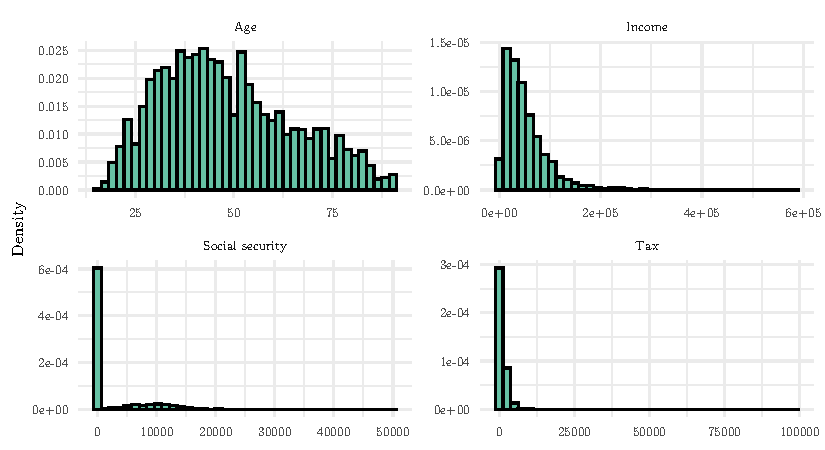
\includegraphics[width=1\textwidth,height=\textheight]{dr-utility-volker-kesteren_files/figure-pdf/fig-vars-orig-1.pdf}

}

\caption{\label{fig-vars-orig}Histograms of the considered subset of
observations and continuous variables in the March 2000 U.S. Current
Population Survey.}

\end{figure}



\end{document}
